\subsection{Network analysis}

Analysing the network of the application proved to be a difficult task. 
In order to only retrieve the network traffic from the android emulator Mitmproxy was used.
Mitemproxy had an issue with the Android emulator where it would constantly fail the TLS handshake. 
This made following the new connections hard. 
In order to properly retrieve the all the in-and outgoing traffic \href{https://github.com/shroudedcode/apk-mitm}{apk-mitm} was used.



\subsubsection{HTTP proxy analysis}

Mitmproxy was able to detect an incoming POST request to an outside IP. 
The POST request would connect with the IP address 172.67.131.170 as seen on figure \ref{tim-mitmrequest}.

\begin{figure}[H]
    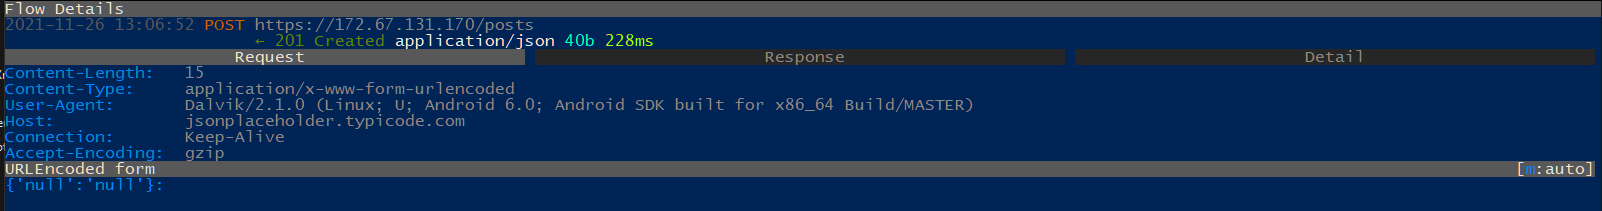
\includegraphics[width=1\textwidth]{mitmreq.png}
    \caption{IP found with mitm}
    \label{tim-mitmrequest}
\end{figure}

\begin{figure}[H]
    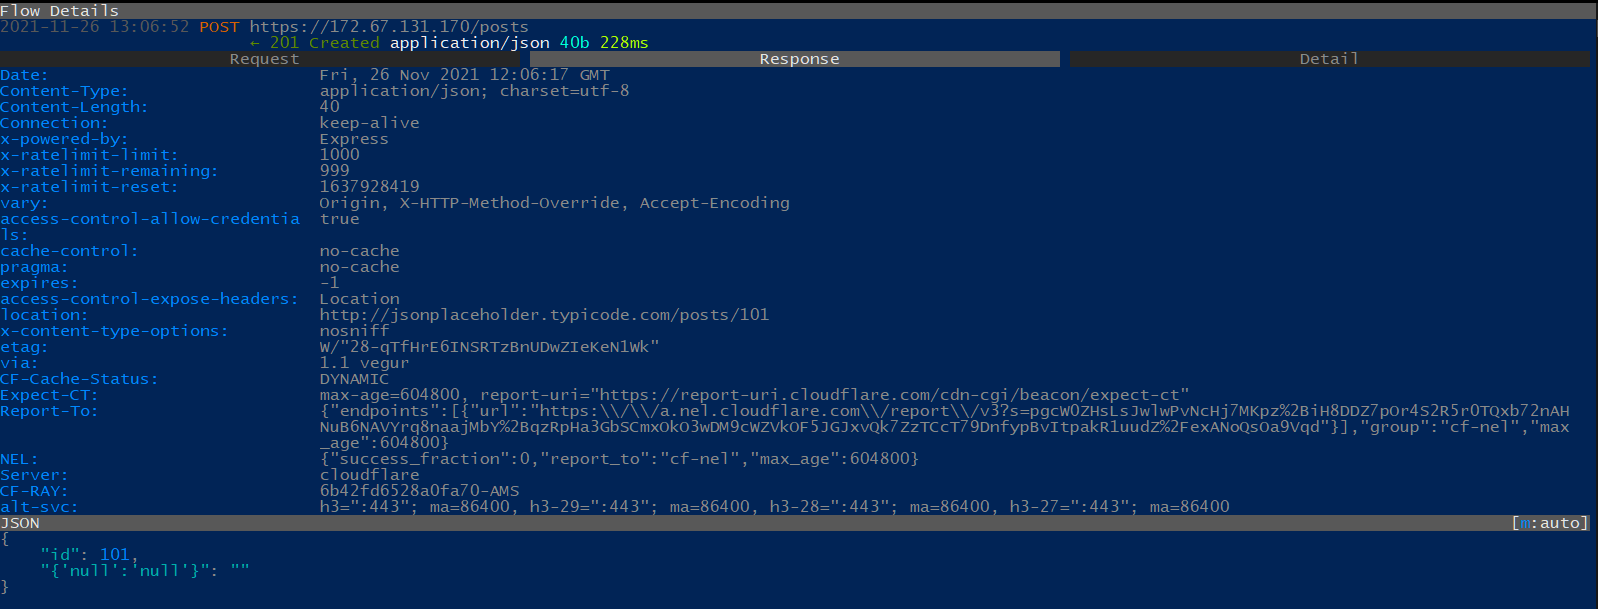
\includegraphics[width=1\textwidth]{networkresponse.png}
    \caption{Response given to the request}
    \label{tim-mitmresponse}
\end{figure}

The POST request contained a JSON file which had an ID with two values. 
The two values however were both null as shown on figure \ref{tim-mitmresponse}.
This was most likely due to an error in the application. 
Also shown on this figure is site that would be sent to.
This site is an online JSON placeholder site.
Any other requests that Mitmproxy picked up were just the expected connections done by google.

\subsubsection{Reconnaissance}

A short Reconnaissance was done on the IP address, Mitmproxy had noted it was an Cloudflare connection.
\href{https://www.shodan.io/host/172.67.131.170}{Shodan} backed this showing that it was indeed owned by Cloudflare, Inc.
There was not much else to go on except for that one connection so company that built the app made sure to cover their tracks.
